\section{Rancangan Sistem Tiket}

\subsection{Komponen Sistem Tiket (tanpa Pengendalian Aliran)}

Komponen sistem tiket dapat dibagi menjadi beberapa bagian, yaitu layanan tiket, basis data relasional, dan kluster Redis. Komponen basis data relasional dapat dibagi menjadi tiga jenis, yaitu kluster PostgreSQL dengan replika baca, kluster CitusData, dan kluster YugabyteDB. Komponen ini yang akan menjadi sumber kebenaran utama dari sistem ini. Selain itu, kluster Redis digunakan untuk menyimpan data agregat ketersediaan berdasarkan area. Arsitektur ini diilustrasikan pada Gambar \ref{fig:ticket-nofc}.

\begin{figure}[H]
    \centering
    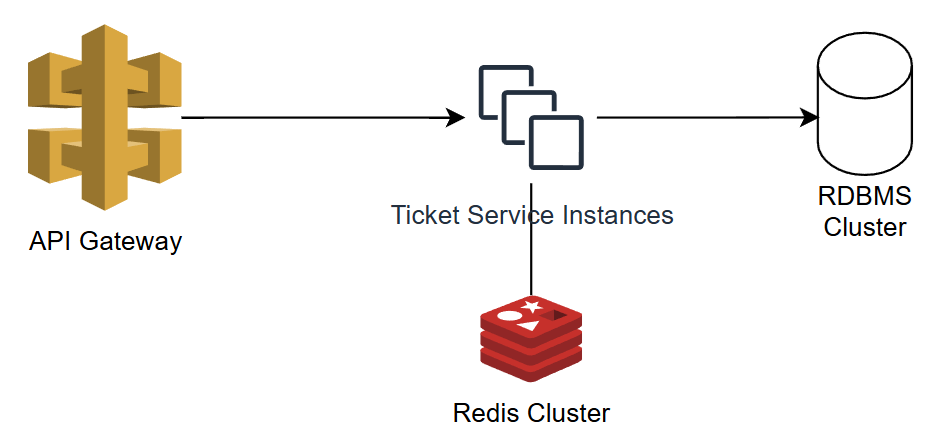
\includegraphics[width=0.8\textwidth]{resources/chapter-3/ticket-nofc.png}
    \caption{Diagram Arsitektur Sistem Tiket Tanpa Pengendalian Aliran}
    \label{fig:ticket-nofc}
\end{figure}

\pagebreak

\subsection{Komponen Sistem Tiket (dengan Pengendalian Aliran)}

Pada sistem tiket dengan pengendalian aliran, terdapat dua komponen baru yaitu RabbitMQ dan pemroses pesanan. RabbitMQ bertugas untuk menyimpan antrean permintaan pemesanan tiket dan pemroses pesanan bertugas untuk memproses pemesanan tiket. Selain itu, kluster Redis memiliki tanggung jawab tambahan untuk menyimpan data yang digunakan untuk menolak permintaan pesanan yang masuk lebih awal. Arsitektur ini diilustrasikan pada Gambar \ref{fig:ticket-fc}.

\begin{figure}[H]
    \centering
    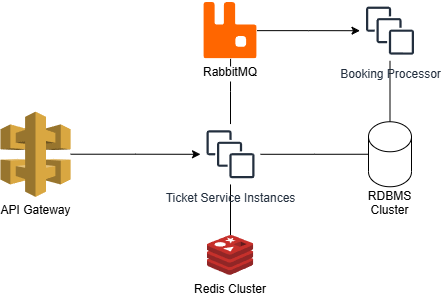
\includegraphics[width=0.8\textwidth]{resources/chapter-3/ticket-fc.png}
    \caption{Diagram Arsitektur Sistem Tiket dengan Pengendalian Aliran}
    \label{fig:ticket-fc}
\end{figure}

\subsection{Variasi Basis Data Relasional}

Untuk membandingkan pendekatan penskalaan yang berbeda, tiga arsitektur basis data diuji. Gambar \ref{fig:rdbms-variation} secara visual membedakan ketiganya: (1) kluster PostgreSQL standar dengan satu \textit{Primary} untuk tulis dan satu \textit{Replica} untuk baca; (2) kluster CitusData dengan satu Citus Coordinator yang mendistribusikan kueri ke beberapa Citus Worker; dan (3) kluster YugabyteDB dengan beberapa \textit{node} Master untuk metadata dan beberapa \textit{node} TServer untuk penyimpanan data.

\begin{figure}[H]
    \centering
    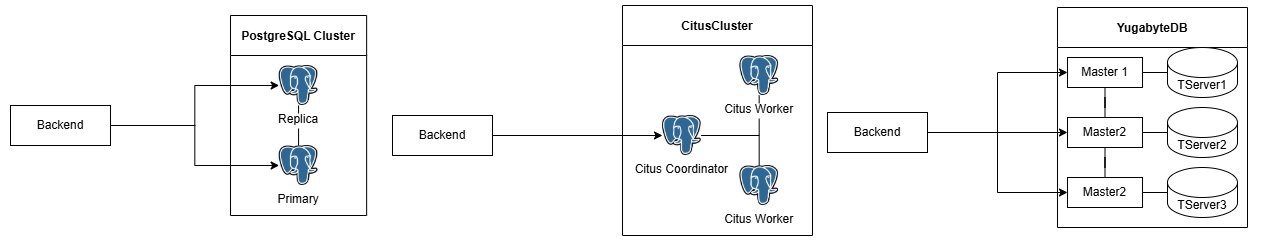
\includegraphics[width=1\textwidth]{resources/chapter-3/rdbms.png}
    \caption{Variasi Basis Data Relasional}
    \label{fig:rdbms-variation}
\end{figure}

Pada konfigurasi kluster PostgreSQL, klien terhubung dengan semua instans. Pada konfigurasi CitusData, klien hanya terhubung dengan koordinator dan koordinator yang akan meneruskan permintaan kepada \textit{worker}. Pada konfigurasi YugabyteDB, klien terhubung dengan semua Master yang masing-masing terhubung dengan TServer. Klien sebenarnya dapat terhubung dengan salah satu master saja, tetapi konfigurasi seperti ini membuat koneksi klien ke YugabyteDB menjadi lebih tahan terhadap kegagalan dan juga dapat mengurangi beban agar tidak terpusat pada satu instans saja.

Konfigurasi kluster PostgreSQL memiliki skalabilitas yang terbatas dengan peningkatan penulisan hanya dapat dicapai dengan penskalaan secara vertikal. Laju penulisan CitusData dan YugabyteDB dapat ditingkatkan dengan menambah jumlah instans.

\textit{Pooler} PGCat akan digunakan agar direct connection basis data yang terbatas dapat digunakan ulang dan dipakai oleh client yang lebih banyak. Selain itu, pada konfigurasi kluster PostgreSQL \textit{pooler} ini berguna sebagai pembagi beban kueri baca antara \textit{primary} dan replika.

\subsection{Integrasi Layanan Pembayaran}

Sistem tiket terintegrasi dengan layanan pembayaran yang disimulasikan (\textit{mock service}). Rancangan layanan ini dibahas pada Lampiran ref{apx:payment-service}.

\subsection{Alur Sistem Tiket}

\subsubsection{Alur Fitur Acara}

Alur untuk berbagai fitur terkait acara diilustrasikan pada Gambar \ref{fig:flow-event}. Diagram ini menunjukkan tiga alur permintaan opsional (opt) dari User ke Ticket Backend:

\begin{enumerate}
    \item Untuk detail acara, sistem langsung melakukan kueri ke Database.
    \item Untuk ketersediaan area secara agregat, sistem mengambil data yang sudah diolah dari Redis, sehingga mengurangi beban pada basis data utama.
    \item Untuk ketersediaan kursi, diagram menunjukkan blok alternatif (alt). Sistem pertama-tama memeriksa cache di memori internal. Jika data ditemukan, data akan langsung dikembalikan (\textit{cache hit}). Jika tidak (\textit{cache miss}), sistem akan melakukan kueri ke Database, menyimpan hasilnya di-\textit{cache} untuk permintaan berikutnya, lalu mengembalikannya ke pengguna.
\end{enumerate}

\begin{figure}[H]
    \centering
    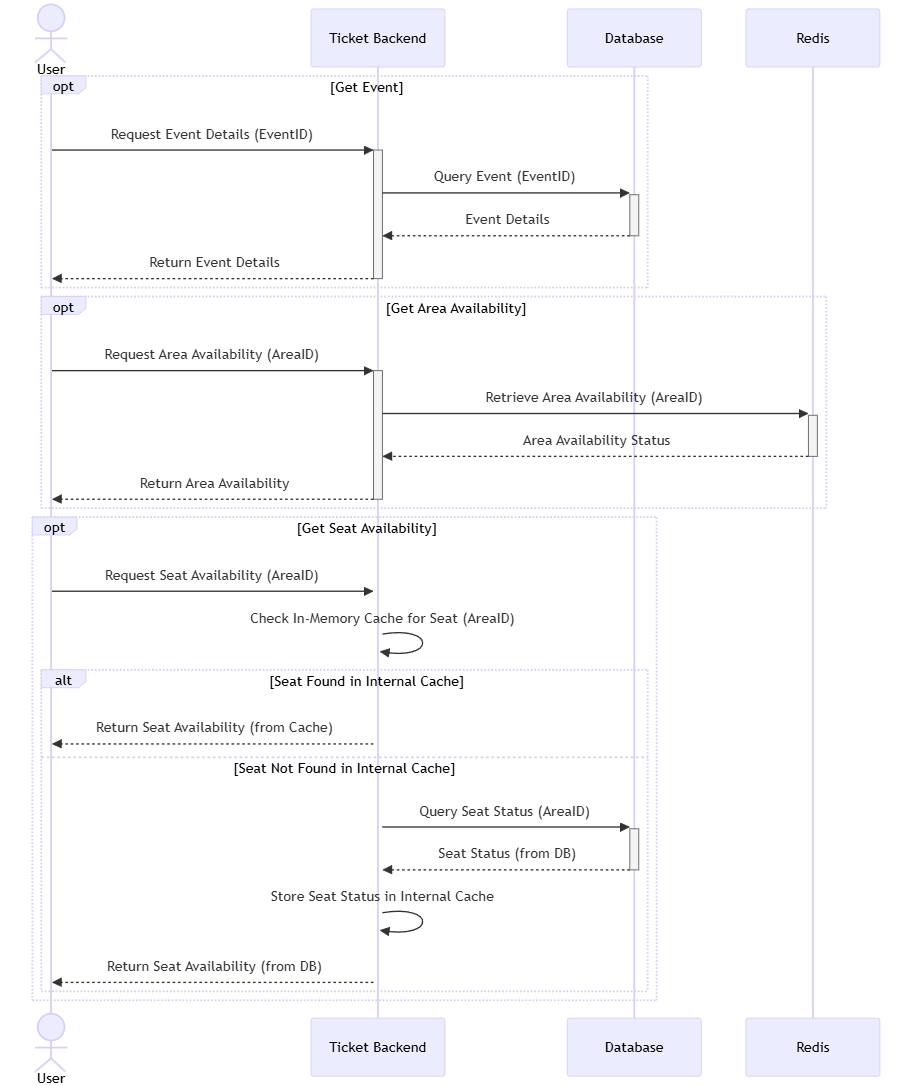
\includegraphics[width=1\textwidth]{resources/chapter-3/event-flow.png}
    \caption{Diagram Alur Fitur acara}
    \label{fig:flow-event}
\end{figure}

\pagebreak

\subsubsection{Alur Fitur Pemesanan Tiket (tanpa pengendalian aliran)}

Proses pemesanan tiket tanpa pengendalian aliran, yang diilustrasikan pada Gambar \ref{fig:flow-book-flow}, dirancang untuk menjaga integritas data. Alurnya adalah sebagai berikut: setelah menerima permintaan, sistem pertama-tama melakukan pengecekan idempotensi di Redis untuk mencegah pemrosesan duplikat. Jika ini adalah permintaan baru, Ticket Backend akan memulai transaksi (Begin Transaction) dengan Database. Langkah krusialnya adalah melakukan kueri penguncian baris (Lock seat rows) untuk memastikan kursi yang dipilih tidak dapat dipesan oleh transaksi lain secara bersamaan. Jika kursi tidak tersedia atau gagal dikunci, transaksi akan dibatalkan (Rollback). Jika berhasil, sistem akan membuat tagihan di Payment Backend, menyimpan informasi pesanan, dan akhirnya melakukan Commit Transaction untuk menyelesaikan pemesanan.

\begin{figure}[H]
    \centering
    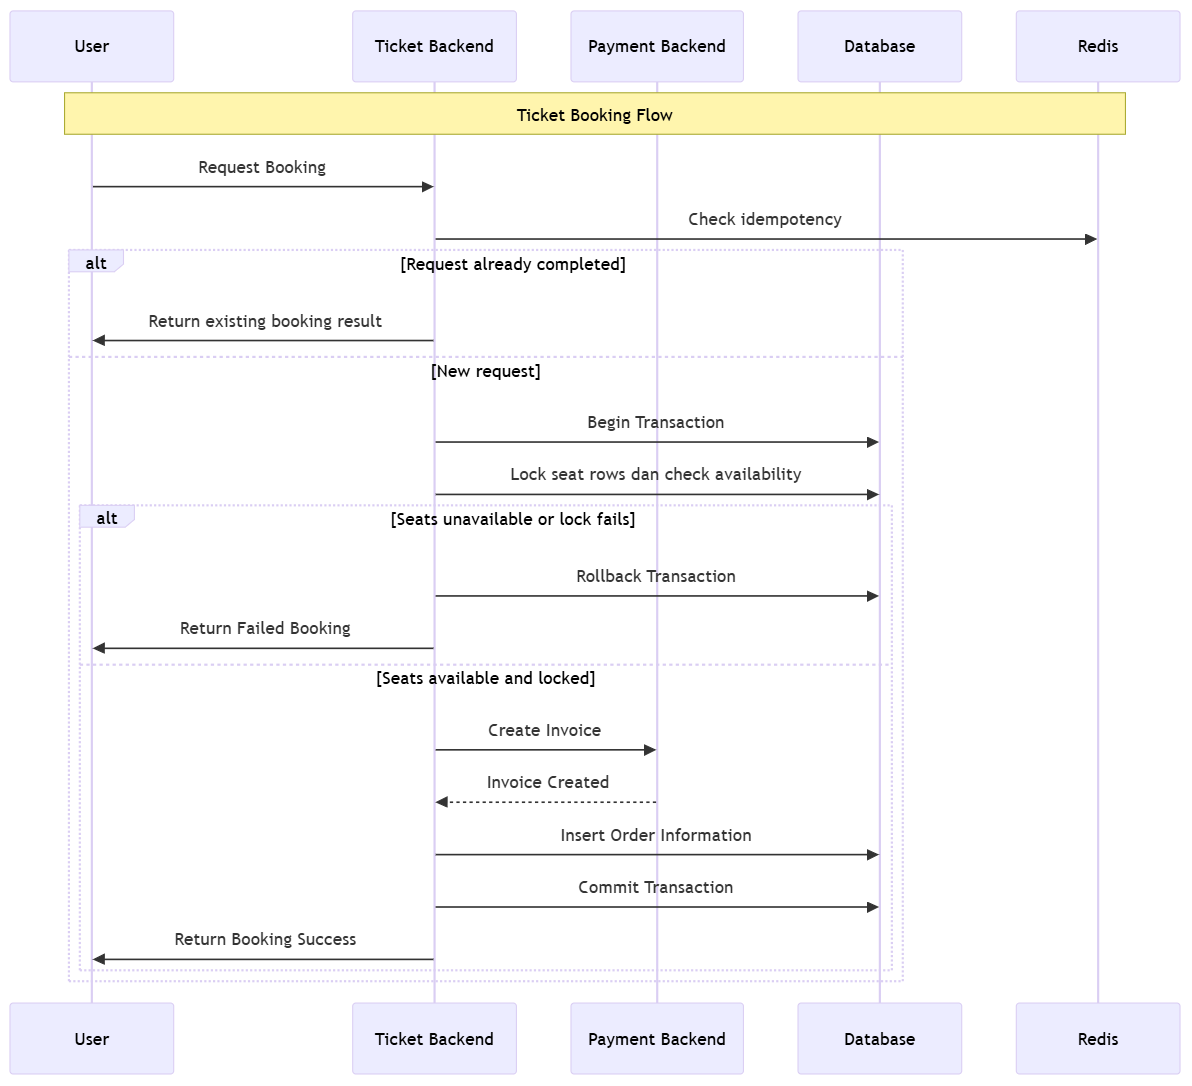
\includegraphics[width=1\textwidth]{resources/chapter-3/book-flow.png}
    \caption{Diagram Alur Fitur Pemesanan Tiket (tanpa pengendalian aliran)}
    \label{fig:flow-book-flow}
\end{figure}

\pagebreak

Alur pembayaran dan konfirmasi tiket, seperti yang ditunjukkan pada Gambar \ref{fig:flow-order-payment-flow}, melibatkan dua proses yang berjalan paralel. Pertama, User berinteraksi langsung dengan Payment Backend untuk membayar tagihan (Pay Invoice). Kedua, dan yang lebih penting, diagram ini menunjukkan proses notifikasi asinkron dalam blok par. Payment Backend secara independen mengirimkan webhook (Notify Payment Status Update) ke Ticket Backend. Bergantung pada status pembayaran, Ticket Backend kemudian akan memperbarui status pesanan, menerbitkan tiket (Insert Published Ticket), dan mengoreksi data agregat ketersediaan di Redis. Pengguna kemudian dapat secara terpisah memeriksa status pesanan mereka, yang sudah diperbarui oleh proses di latar belakang ini.

\begin{figure}[H]
    \centering
    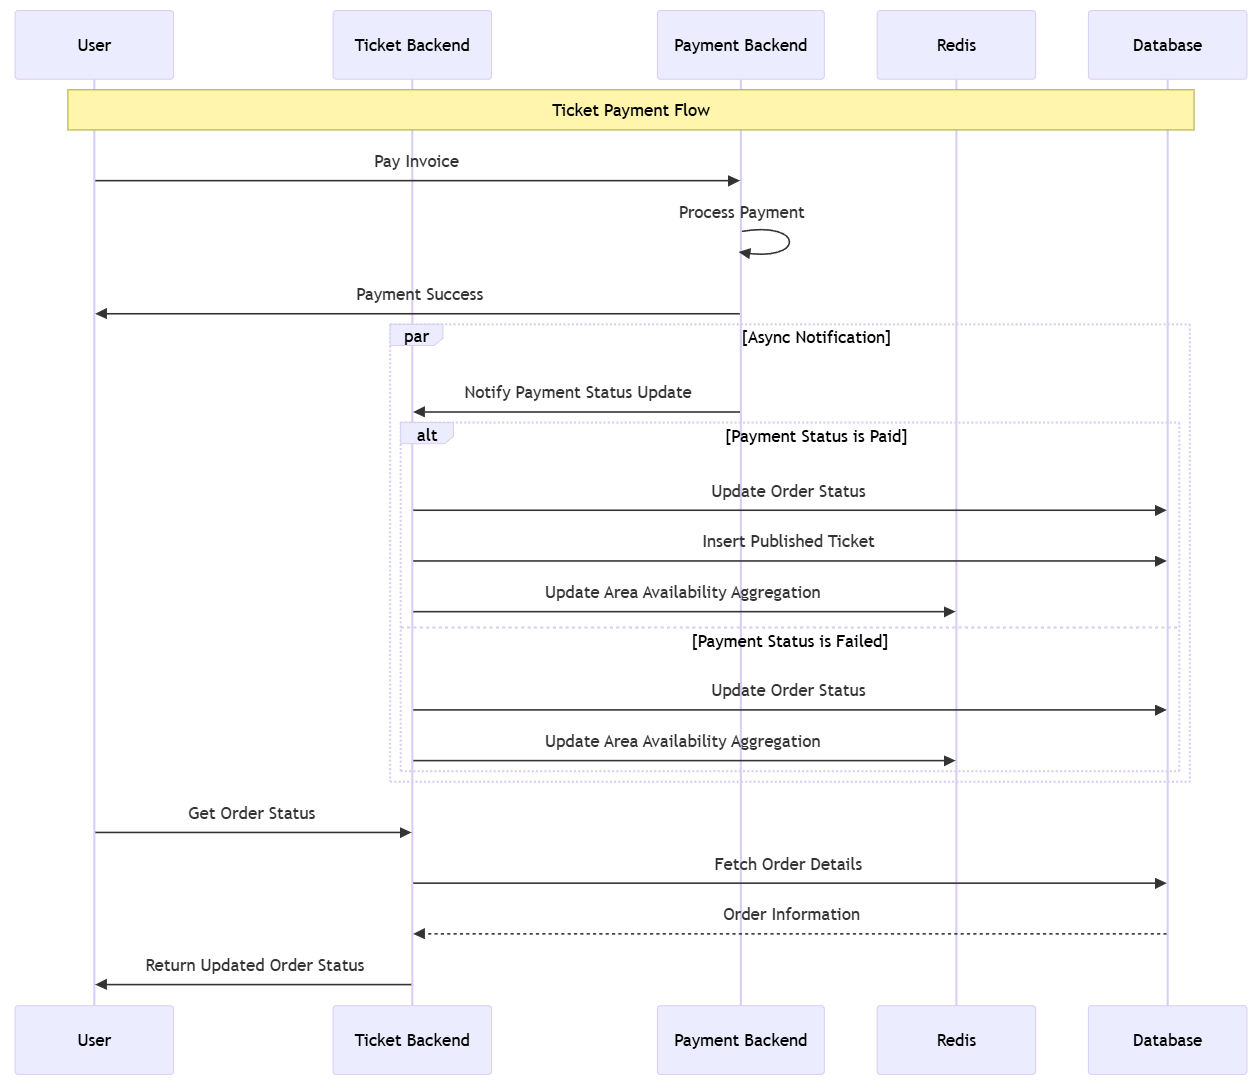
\includegraphics[width=1\textwidth]{resources/chapter-3/order-payment.png}
    \caption{Diagram Alur Fitur Pembayaran Tiket (tanpa pengendalian aliran)}
    \label{fig:flow-order-payment-flow}
\end{figure}

\pagebreak

\subsubsection{Alur Fitur Pemesanan Tiket (dengan pengendalian aliran)}

Alur pemesanan tiket dengan pengendalian aliran, yang dirinci pada Gambar \ref{fig:flow-book-fc}, memperkenalkan antrean untuk mengatur beban ke basis data. Prosesnya sebagai berikut: setelah cek idempotensi, sistem melakukan pengecekan kedua di Redis untuk menolak permintaan lebih awal jika kursi yang sama sedang dalam proses pemesanan lain. Jika lolos, Ticket Backend tidak langsung ke basis data, melainkan mempublikasikan permintaan ke antrean di RabbitMQ dan menunggu pesan balasan. Di sisi lain, sebuah Ticket Worker mengambil pesan dari antrean tersebut (bagian "Worker Processing"). Worker inilah yang bertanggung jawab menjalankan transaksi basis data yang intensif (mengunci baris, membuat tagihan, dan commit). Setelah selesai, worker mengirimkan hasilnya kembali melalui antrean balasan, yang kemudian diterima oleh Ticket Backend dan diteruskan kepada User. Alur ini mengubah pemrosesan yang tadinya sinkron menjadi asinkron untuk menjaga stabilitas.

\begin{figure}[H]
    \centering
    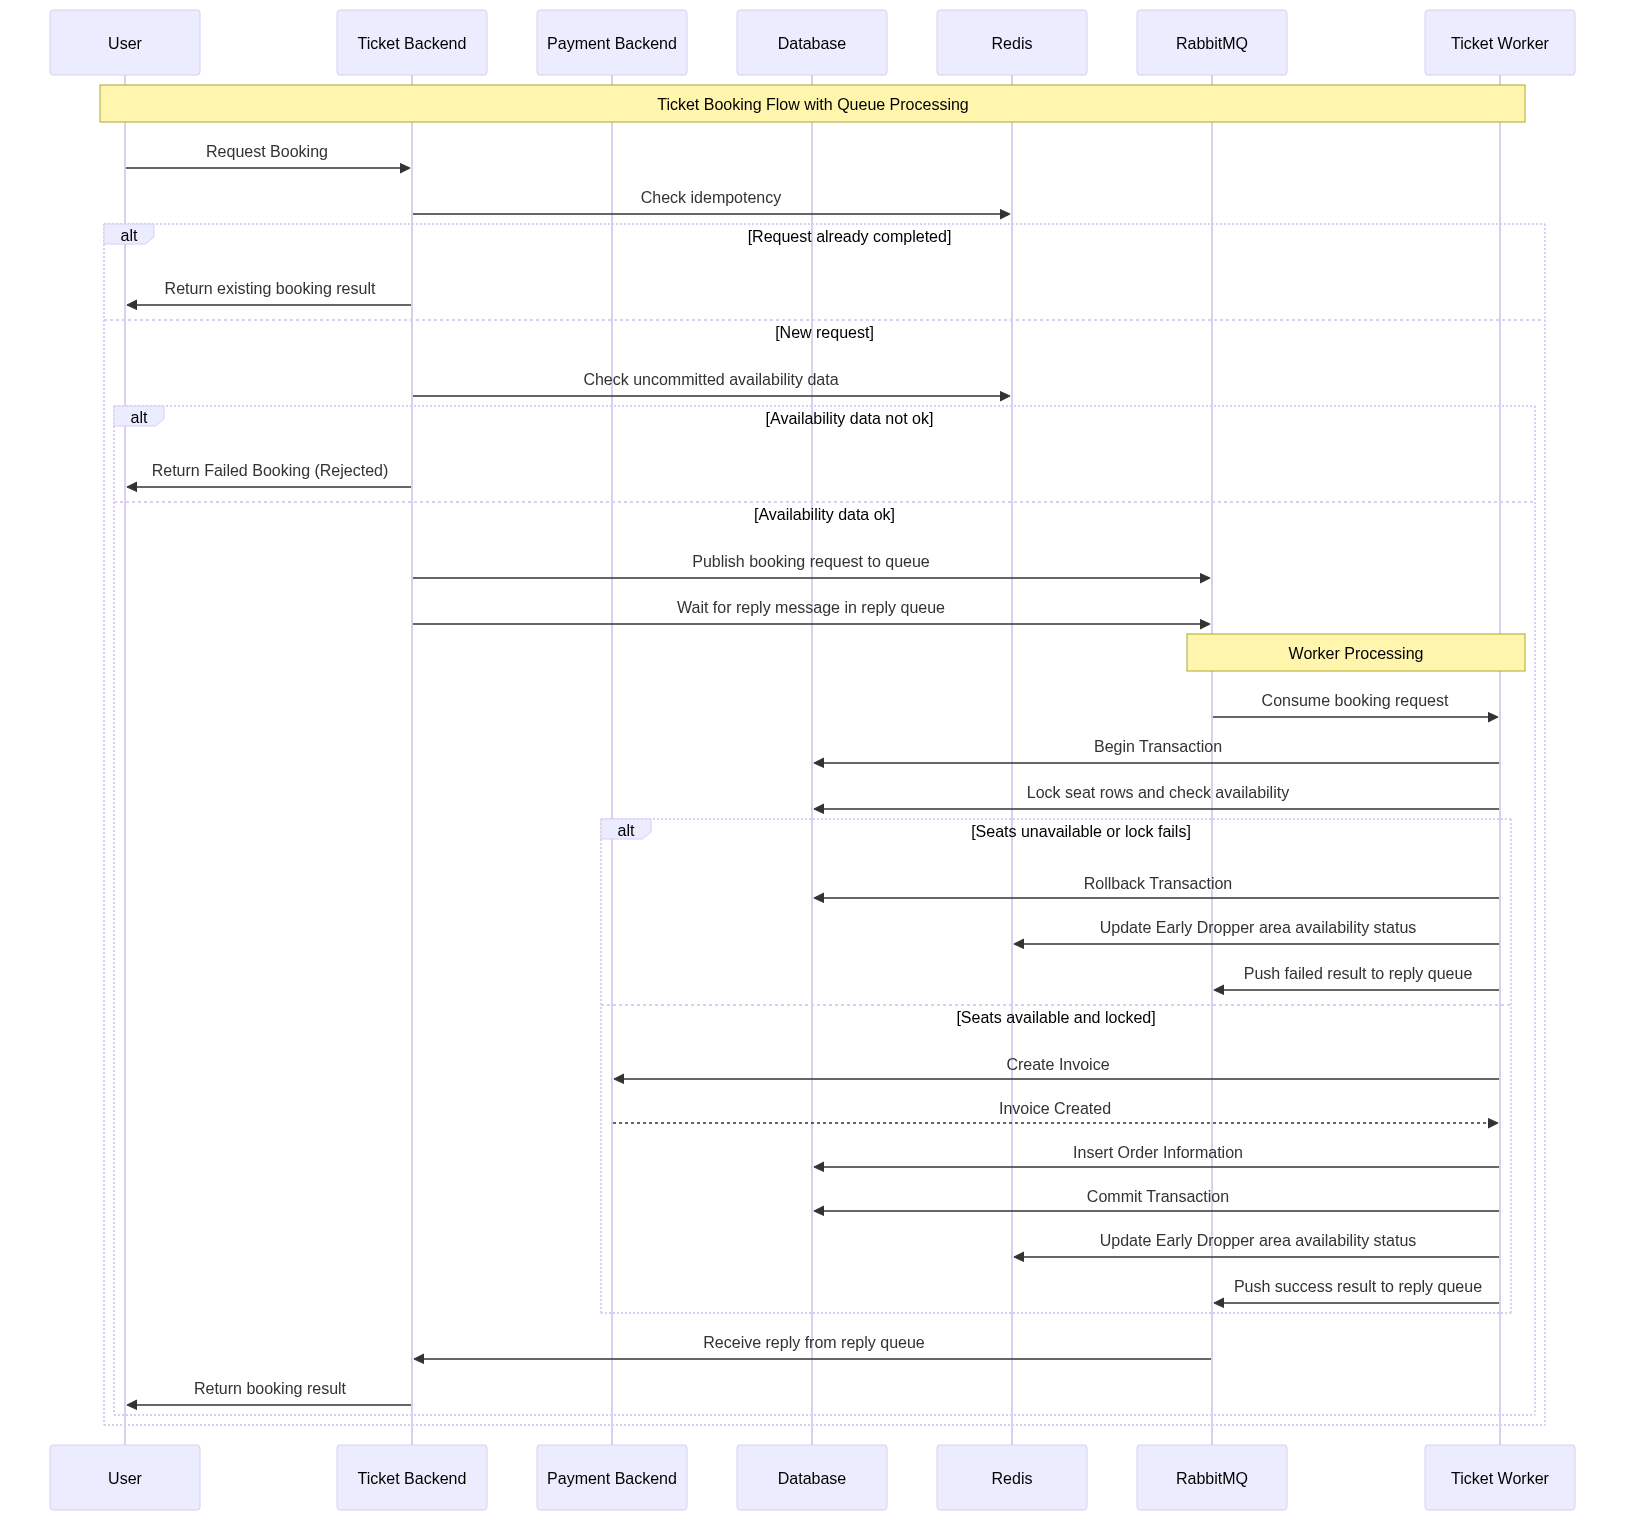
\includegraphics[width=1\textwidth]{resources/chapter-3/book-async.png}
    \caption{Diagram Alur Fitur Pemesanan Tiket (dengan pengendalian aliran)}
    \label{fig:flow-book-fc}
\end{figure}

\pagebreak

Ketika pengguna berhasil memesan, pengguna akan melakukan pembayaran kepada gerbang pembayaran. Setelah pembayaran selesai, pengguna memeriksa status pesanan yang telah dibuat. Tidak ada perbedaan signifikan selain pembaruan data pada Redis untuk sinkronisasi data yang menjadi basis untuk menolak permintaan pesanan lebih awal. Alur fitur ini diilustrasikan pada Gambar \ref{fig:flow-order-payment-fc}.

\begin{figure}[H]
    \centering
    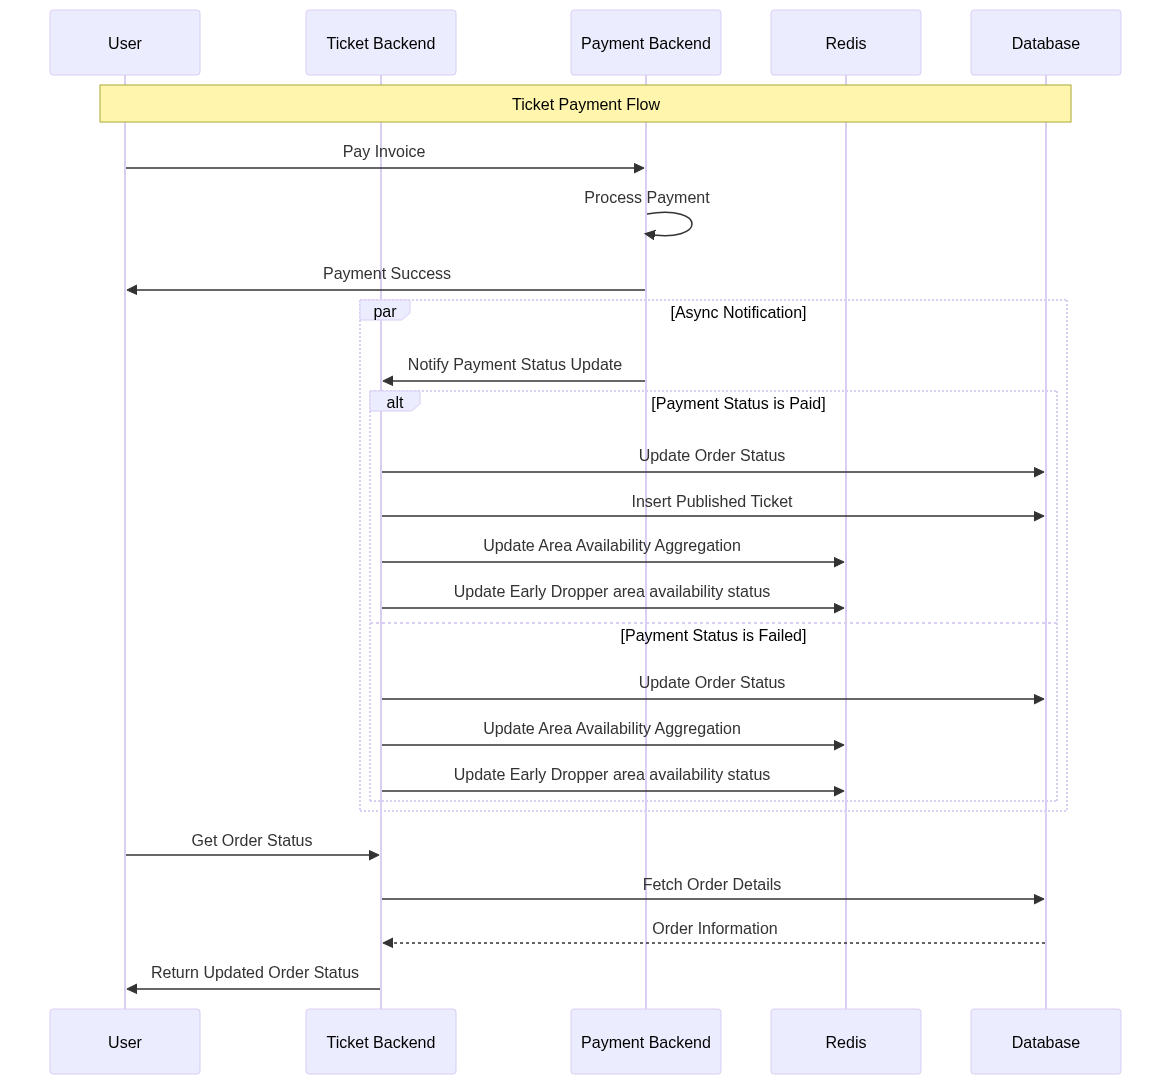
\includegraphics[width=1\textwidth]{resources/chapter-3/order-payment-fc.png}
    \caption{Diagram Alur Fitur Pembayaran Tiket (dengan pengendalian aliran)}
    \label{fig:flow-order-payment-fc}
\end{figure}

\pagebreak

\subsubsection{Alur Fitur Pembacaan Pesanan}

Terdapat dua operasi tambahan yang berkaitan dengan pembacaan pesanan, yaitu membaca detail pesanan dan membaca tiket yang sudah diterbitkan. Alur fitur ini diilustrasikan pada Gambar \ref{fig:flow-order-flow}.

\begin{figure}[H]
    \centering
    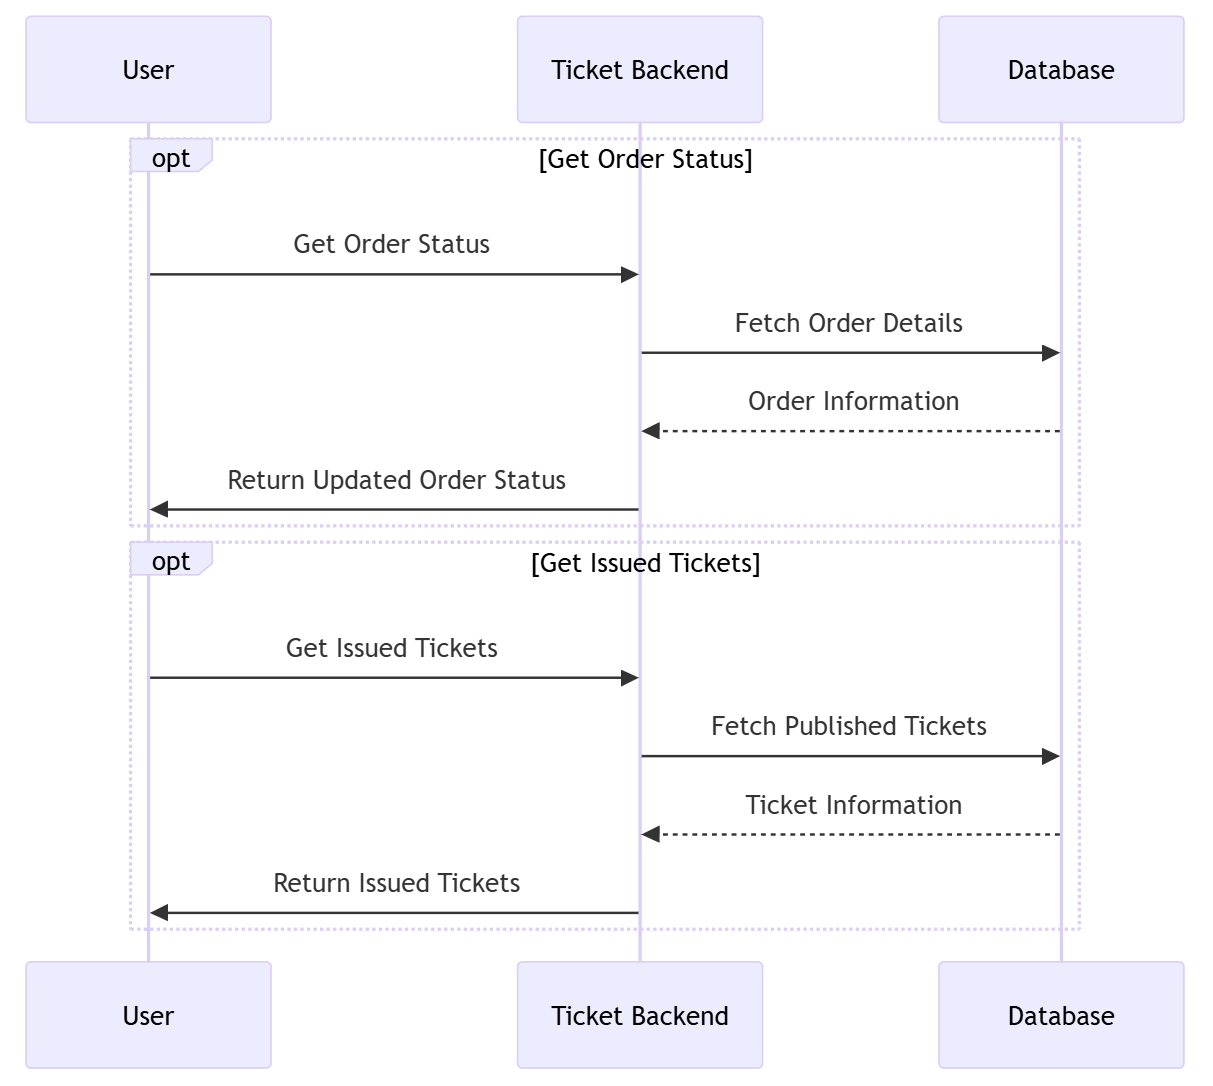
\includegraphics[width=1\textwidth]{resources/chapter-3/order-flow.png}
    \caption{Diagram Alur Fitur Pembacaan Pesanan}
    \label{fig:flow-order-flow}
\end{figure}